%%%%%%%%%%%%%%%%%%%%%%%%%%%%%%%%%%%%%%%%%
% Journal Article
% LaTeX Template
% Version 1.4 (15/5/16)
%
% This template has been downloaded from:
% http://www.LaTeXTemplates.com
%
% Original author:
% Frits Wenneker (http://www.howtotex.com) with extensive modifications by
% Vel (vel@LaTeXTemplates.com) and Fabio Mendes (f.mendes@auckland.ac.nz)
%
% License:
% CC BY-NC-SA 3.0 (http://creativecommons.org/licenses/by-nc-sa/3.0/)
%
%%%%%%%%%%%%%%%%%%%%%%%%%%%%%%%%%%%%%%%%%

%----------------------------------------------------------------------------------------
%	PACKAGES AND OTHER DOCUMENT CONFIGURATIONS
%----------------------------------------------------------------------------------------

%\documentclass[oneside,twocolumn]{article}
\documentclass[oneside]{article}

\usepackage{blindtext} % Package to generate dummy text throughout this template 

\usepackage{graphicx} % FKM: for figures
\usepackage{color} % FKM: for colored text
\usepackage{float} % FKM: for forcing figure placement
\usepackage[breakable]{tcolorbox} % FKM: for text box
\usepackage{enumerate} % FKM: for bullet point lists
\usepackage{setspace} % FKM: line spacing
\usepackage[margin=1in]{geometry} % FKM: margins

\usepackage[sc]{mathpazo} % Use the Palatino font
\usepackage[T1]{fontenc} % Use 8-bit encoding that has 256 glyphs
% \linespread{1.05} % Line spacing - Palatino needs more space between lines
\usepackage{microtype} % Slightly tweak font spacing for aestheticsgins
\usepackage[small,labelfont=bf,up,up]{caption} % Custom captions under/above floats in tables or figures
\usepackage{booktabs} % Horizontal rules in tables
\usepackage{amsmath} % Text in equations

\usepackage[shortlabels]{enumitem} % customized lists (shortlabels
                                % necessary to have i., ii., etc., in enumerate)
\setlist[itemize]{noitemsep} % Make itemize lists more compact

\usepackage{abstract} % Allows abstract customization
\renewcommand{\abstractnamefont}{\normalfont\bfseries} % Set the "Abstract" text to bold
\renewcommand{\abstracttextfont}{\normalfont\small\itshape} % Set the abstract itself to small italic text

\usepackage{titlesec} % Allows customization of titles

\usepackage{fancyhdr} % Headers and footers
\pagestyle{fancy} % All pages have headers and footers
\fancyhead{} % Blank out the default header
\fancyfoot{} % Blank out the default footer
\fancyhead[C]{Authors et al. $\bullet$ August 2018 $\bullet$ bio{\color{red}R}$\chi$ve} % Custom header text
\fancyfoot[RO,LE]{\thepage} % Custom footer text

\usepackage{titling} % Customizing the title section

\usepackage[hidelinks]{hyperref} % For hyperlinks in the PDF

\usepackage{natbib}
\bibliographystyle{apalike}

\setlength\columnsep{20pt}

%----------------------------------------------------------------------------------------
%	TITLE SECTION
%----------------------------------------------------------------------------------------

\setlength{\droptitle}{-4\baselineskip} % Move the title up

\pretitle{\begin{center}\Huge\bfseries} % Article title formatting
\posttitle{\end{center}} % Article title closing formatting
\title{How to validate your probabilistic model implementation} % Article title
\author{\textsc{An author here$^{1,2*}$}, \textsc{Another author
    here$^{1*}$}, \\ \textsc{Yet another author here$^{1*}$},
  \textsc{Last author here$^{1*}$} \\
\small $^1$School of Computer Science, The University of Auckland\\
\small $^2$School of Biological Sciences, The University of Auckland\\
\small
\href{mailto:f.mendes@auckland.ac.nz}{Corresponding authors$^*$: f.mendes@auckland.ac.nz,}
\href{mailto:f.mendes@auckland.ac.nz}{another.email@auckland.ac.nz}
%\and % Uncomment if 2 authors are required, duplicate these 4 lines if more
%\textsc{Jane Smith}\thanks{Corresponding author} \\[1ex] % Second author's name
%\normalsize University of Utah \\ % Second author's institution
%\normalsize \href{mailto:jane@smith.com}{jane@smith.com} % Second author's email address
}
\date{\today} % Leave empty to omit a date
\renewcommand{\maketitlehookd}{%
\begin{abstract}
  \noindent Biology has become a highly mathematical discipline in
  which probabilistic models play a central role,
  and as a result its research is now dependent on computational tools
  capable of carrying out complex analyses.
  These tools must be not only efficient, but also correctly
  implemented.
  Both goals are difficult to achieve for several reasons, such as the
  multidisciplinary nature of method development, and a still
  embrionary literature on good software development and statistical
  practices aimed at professionals from disparate fields.
  Here we provide guidelines for the validation of probabilistic model
  implementations, focusing on Bayesian approaches.
  This manuscript summarizes good practices for assessing the correctness of
  simulation and inference procedures under a model, and is
  accompanied by a living document with examples to aid researchers
  developing Bayesian methods.
\end{abstract}
}

%----------------------------------------------------------------------------------------

\doublespacing

\begin{document}

% Print the title
\maketitle

%----------------------------------------------------------------------------------------
%	ARTICLE CONTENTS
%----------------------------------------------------------------------------------------

\section*{Introduction}
The last two decades have seen the biological sciences undergo a major revolution.
Critical technological innovations such as the advent of massive parallel sequencing and the accompanying improvements in computational power and storage have flooded biology with unprecedented amounts of data ripe for analysis.
Not only has intraspecific data from multiple individuals allowed
progress in disparate fields like medicine and epidemiology
\citep[e.g.,][]{1000g,humanmicrobiome,neafsey15}, population genetics \citep[e.g.,][]{lynch07,lack16,demanuel16} and disease ecology \citep[e.g.][]{rosenblum13,bates18}, but now a large number of species across the tree of life have had their genomes sequenced, furthering our understanding of species relationships and diversification \citep[e.g.,][]{martin13,brawand14,jarvis14,novikova16,pease2016,kawahara19,upham19}.
However, as the old adage goes, with great power comes great responsibility: never has the data available to the average biologist been so abundant, but also never has one been so aware of both its complexity and the necessary care with which to analyze it.
Almost at par with with data accumulation is the rate at which new computational tools are being proposed, as evidenced by journals entirely dedicated to method advances, methodological sections in biological journals, and computational biology degrees being offered by institutions around the world.

One extreme case is the discipline of evolutionary biology (on which we focus our attention).
While it could be said that many decade-old questions and hypotheses
in evolutionary biology have aged well and stood up the test of time
(e.g., the Red Queen hypothesis,
\citealt{vanvalen73,lively87,morran11,gibson15}; the
Bateson-Dobzhansky-Muller model, \citealt{dob36,muller40,hopkins12,roda17}), data analysis
practices have changed drastically in recent years, to the
point they would likely seem obscure to an evolutionary biologist last active 40 years ago.
In particular, evolutionary biology has become highly statistical, with the development and utilization of models now being commonplace.

Models are employed in the sciences for many reasons, and fall within
a biological abstraction continuum \citep{servedio14}, going from
fully verbal, highly abstract models (e.g., \citealt{vanvalen73}), through proof-of-concept models
that formalize verbal models (e.g., \citealt{maynard78,reinhold99,mendes18}), to probabilistic models that interact
directly with data (i.e., models with a likelihood function such as \citealt{yule24,felsenstein73,hky,hudson90}).
Though mathematical models are in general more frequently used in
evolutionary biology, there has been a sharp surge in instances of the
latter cases (i.e., probabilistic models) in conjunction with computational tools implementing them
(Fig. 1).

Despite the increasing pervasiveness of probabilistic models in the
biological sciences, tools implementing such models show large
variation not only with respect to code quality (from a software engineering
perspective), but also correctness \citep{darriba18}.
This is unsurprising given the multidisciplinary nature of model and method
development, and the challenges inherent to software research funding
\citep{siepel19}.
The bioinformatics community is thus in dire need of resources that
provide guidance for code improvement and validation.

Here, we summarize best practices in probabilistic  model validation for method
developers, with an emphasis on Bayesian methods.
We hope our guidelines can help raise the standards for software
package releases required by users, developers and reviewers alike,
and consequently lead to computational tools that are more efficient, better documented, and most
importantly, correctly implemented.

% \begin{figure}
%   \includegraphics[width=\linewidth]{fig1}
%   \caption{Hemiplasy on species trees and gene trees.
%     Panel (a) shows substitutions that occur on each of the two discordant gene trees, and the corresponding site patterns produced.
%     (b) Incorrectly inferred convergent substitutions (from the site patterns produced in [a]) when analyses are conducted on the species tree topology.
%     (c) Incorrectly inferred convergent substitutions when analyses are conducted on the CDS tree (discordant tree topology 2).}
%   \label{fig:1}
% \end{figure}

%------------------------------------------------

\section*{Probabilistic model validation}

The central component of a probabilistic model is its likelihood
function, $\text{P}(D|\theta)$, which establishes the
interface between an abstract representation of reality (defined by parameters $\theta$), and the
empirical world (from which data $D$ is obtained).
In a frequentist statistical framework, the likelihood function is the sole
component of a probabilistic model.
Here, tasks like parameter estimation and model comparison are conducted
by maximizing the likelihood function across parameter
space.

In Bayesian inference, on the other hand, a probabilistic model $M$
defines a posterior probability distribution for its parameters,
$\text{P}(\theta|D) = \frac{\text{P}(D|\theta)\text{P}(\theta)}{\text{P}(D)}$, in which our prior
knowledge or beliefs about the natural world -- represented by the prior
distribution $\text{P}(\theta)$ -- are confronted and updated by the data through the
likelihood function.
$\text{P}(D) = \int_\theta \text{P}(D|\theta)\text{P}(\theta)d\theta$, the probability of
the data, is also known as the marginal likelihood or the model
evidence.
Crucially, note that a Bayesian model includes a prior, $\text{P}(\theta)$:
when models are compared, for example, $\text{P}(\theta)$ needs to be taken
into account when computing the model evidence $\text{P}(D)$.

Under simple-enough models, the probability density function of the posterior distribution can sometimes be analytically
derived.
Models routinely used in biology are nonetheless often complex enough
to preclude such closed-form solutions, mainly due to the
intractability of the integral that appears in the marginal
likelihood.
In those cases, techniques like Markov chain Monte Carlo (MCMC) are
routinely employed to sample the posterior distribution, as it uses
the fact that $\text{P}(D)$ evaluates to a constant that can be
conveniently ignored (i.e., $\text{P}(\theta|D) \propto
\text{P}(\theta|D)\text{P}(\theta)$).
In practice, the algorithm that generates the Markov chain under MCMC is called
Metropolis-Hastings \citep{mh}, and it samples the posterior distribution by
means of a transition mechanism. 
If the resulting chain is long enough, aperiodic, irreducible and
positive recurrent, then the sampled posterior distribution will
approximate the true, target distribution $\text{P}(\theta|D)$
\citep{mau99,gelman}.

We focus on MCMC as the chosen technique for obtaining $\text{P}(\theta|D)$
under an implementation of model $M$,
and a thorough validation effort thus entails verifying the
correctness of (i) the model (i.e., $\text{P}(D|\theta)\text{P}(\theta)$), and (ii)
the components involved in the MCMC transition mechanism.
This is not to say the latter are part of the model (they are
\emph{not}), as it is possible to sample $\text{P}(\theta|D)$ with importance sampling, Hamiltonian
Monte Carlo \citep{hmc}, or even by converting the sampling problem into an
optimization one \citep{zhang18}.

Finally, we stress that we are interested in practices for verifying model
\emph{correctness}.
Determining that one or more independent Markov chains converged on very
similar posterior distributions is not a correctness test, as those
distributions might be very different from the target distribution.
Similarly, obtaining ``reasonable'' results from real data sets also
does not consist of a correctness test, as the true target
distribution (across all parameters) is unknown.

\subsection*{Validating model $M$}

When a model $M$ is implemented for the first time, usually both an
inferential engine, $I(M)$, and a simulator, $S(M)$, need to be devised.
These generate the aforementioned posterior distribution,
$\text{P}_{\text{I}}(\theta|D)$ (we introduce subscript ``I'' for
\textbf{i}nference), and a ``target'' distribution $\text{P}_{\text{S}}(\theta|D)$ (``S''
for \textbf{s}imulation), respectively.
Here, we refer to the distribution produced through simulation as the
target distribution because simulators are used to establish an
expected, ``true'' distribution to be approximated by sampling through MCMC.
Ultimately, we want $\text{P}_{\text{I}}(\theta|D)$ to reach stationarity at
$\text{P}_{\text{S}}(\theta|D)$.

\subsubsection*{Validating the simulator, $S(M)$}\label{verify-correctness-of-simulator-implementation}

As mentioned above, the main purpose of a simulator $S(M)$ in the context of model
validation is to generate a known distribution,
$\text{P}_{\text{S}}(\theta|M)$, that should act as the target distribution during
Bayesian inference.
However, simulators themselves need to be validated.
In the case of models that have well-known parametric distributions as their
likelihood functions (see Box 1), one can validate $S(M)$ by
drawing a very large sample of points and comparing summary statistics
(e.g., mean, variance, etc.) from the sample against their true value counterparts (i.e., the
values used in the simulation procedure). 

Alternatively, summary statistic expectations derived under other kinds of models can also be compared
to those computed from simulated datasets.
One such model is the Yule process \citep{yule24}, also known as a pure-birth model.
The Yule process is a continuous-time Markov process that has been
classically employed in phylogenetics, as a way to model the number of
species in a clade \citep{yule24,aldous01}.
Under the Yule process, for example, the expected tree height,
$\text{E}[t_{MRCA}]$ for a tree with $n$ tips is:

\begin{equation}
  \text{E}[t_{MRCA}] = \sum_{i=2}^{n}\frac{1}{1\lambda}
  \label{eq:yule}
\end{equation}

\noindent where $\lambda$ is the species ``birth'' rate \citep{yule24}.
This analytical expectation can then be compared to the expected tree
height in several independent datasets of simulated phylogenetic trees.
If $S(M)$ was correctly implemented, $\text{E}[t_{MRCA}]$ should be contained within $\pm 2$ standard errors of
the mean in $\sim 95\%$ of all the simulated datasets under the Yule process.

Here, we note that $S(M)$ represents a \emph{direct} simulator (Table
\ref{tab:sim}) of model
$M$ -- i.e., $S(M)$ allows one to directly draw truly independent
samples from $M$.
This is contrast with other simulation strategies, such as conducting
MCMC under a model with fixed parameter values and no data.
This latter approach is predicated on the existence of a correct
implementation of both $I(M)$ and proposal functions, and for this
reason is more appropriately used in the validation of these components rather than in
the validation of $S(M)$ (see below).

\begin{center}
  \begin{table}
  \caption{A non-exhaustive list of direct simulation software commonly used in evolutionary
    biology analyses.}
  \label{tab:sim}
  \centering
  \begin{tabular}{ p{0.7in} | p{1.3in} | p{1in} | p{1.1in} }
    \hline
    Software package & Model type & Platform & Reference \\
    \hline  
    Seq-Gen & Molecular sequence evolution models & Standalone & \citealp{rambaut97} \\
    ms & Coalescent model & Standalone & \citealp{hudson02}\\
    SLiM & Population genetic models & Standalone & \citealp{haller19}\\
    TreeSim & Birth-death models & R & \citealp{stadler11}\\
    mvMORPH & Continuous trait evolution models & R &
                                                      \citealp{clavel15}\\
    phytools & Several phylogenetic models & R & \citealp{revell12}\\
    MASTER & Continuous-time Markov (tree) models & BEAST 2 & \citealp{vaughan13}\\
    \hline
  \end{tabular}
  \end{table}
\end{center}

% \begin{tcolorbox}[breakable, width=12cm, colback=gray!10, boxrule=0pt,
%   break at=11cm/0cm, title=Box 1: Models with well-known parametric \emph{pdf}'s, fonttitle=\bfseries]
\begin{tcolorbox}[breakable, width=\textwidth, colback=gray!10, boxrule=0pt,
  title=Box 1: Models with well-known parametric \emph{pdf}'s, fonttitle=\bfseries]
  \small 
  One commonly used model in macroevolution, specifically in the study
of continuous traits, is a diffusion model known as
Brownian motion (BM; \citealt{felsenstein73}).
The log-likelihood function of this model is simply the multivariate
normal (MVN) probability density function:

\begin{equation}
  \begin{split}
    \text{log P}(\mathbf{y} \mid \mathbf{y_0}, r, \mathbf{T}) = -\frac{1}{2} \Big[ n\text{log}(2\pi) + \text{log}|r \mathbf{T}| \Big] & \\
    -\frac{1}{2} \Big[ (\mathbf{y} - \mathbf{y_0})^T (r \mathbf{T})^{-1} (\mathbf{y} - \mathbf{y_0}) \Big],
  \label{eq:bm}
  \end{split}
\end{equation}

\noindent where $\mathbf{y}$ corresponds to the mean trait values in $n$ species,
$\mathbf{y_0}$ is the trait value at the root of the species tree, $r$ is the variance of the process
(also known as the evolutionary rate, and sometimes represented by $\sigma^2$), and $r\mathbf{T}$ is the
variance-covariance matrix ($\mathbf{T}$ is a matrix whose elements
come from the species tree branch lengths; see Fig. 1 below).

\vspace{.25cm}
The MVN density function describes the distribution that would result from an infinite
number of BM process ``experiments'' (each experiment being non-mean-reverting, and
representing an independent evolutionary trajectory).
Under this model $\theta = \{\mathbf{y_0},
r\}$ and $D = \{\mathbf{y, \mathbf{T}} \}$ (but note that $\mathbf{T}$ can
be a parameter elsewhere in a hierarchical model of which BM is just a
component).

\begin{center}
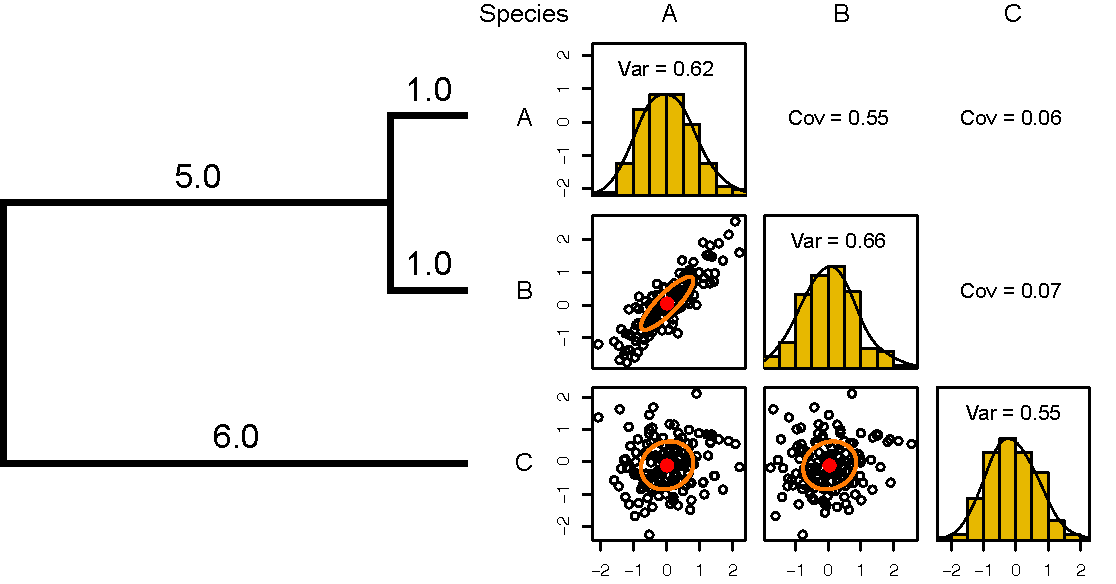
\includegraphics[width=11cm]{../figures/bmsim.pdf}
\label{fig:bmsim}
\captionof{figure}{A sample of 200 draws from a MVN distribution, each
  representing the evolutionary trajectory of one continuous trait along
  the species tree on the left. The root trait value, $\mathbf{y_0}$, and the
  evolutionary rate of the process, $r$, were set to 0.0 and 0.1, respectively. The panel on the right shows
  histograms of trait values sampled from the MVN for each species, as
well as their covariation.}
\end{center}

\vspace{.25cm}
\emph{Validating a BM simulator}

Because the MVN is a \textbf{known parametric
  distribution}, it is trivial to verify the correctness of a
BM model simulator, $S(BM)$.
Figure 1 shows the result of 200 simulations under the MVN
with $\mathbf{y_0} = [0.0, 0.0, 0.0]$, $r = 0.1$, along the tree shown on
the left, which determines the variance-covariance matrix:

\begin{equation}
  r\mathbf{T} = 0.1
  \begin{bmatrix}
    6 & 5 & 0\\
    5 & 6 & 0\\
    0 & 0 & 6
  \end{bmatrix}
  \label{eq:mat}
\end{equation}

One can then see that the simulated variances for the three species
and the covariances between them closely match their true counterparts
(Eq. 3 and the right panel in Fig. 1).
Additionally, the simulated mean trait values in each species fall
within $\pm 2$
standard errors of the mean (see main text).

\vspace{.25cm}
\emph{Validating a BM likelihood implementation}

For a small tree, the likelihood of a set
of parameter values $\theta$ given some observed data is
straightforward to compute (following Eq. \ref{eq:bm}) and can be compared to
the output of a focal implementation.
Interestingly, the likelihood of the BM model can also be computed using a
dynamic-programming algorithm known in the phylogenetics literature
as the ``pruning'' or ``peeling'' algorithm \citep{felsenstein73}.
Thus, if a BM model is implemented correctly, the resulting likelihood
of $\theta$ should match the solution of equation 2 no matter
which algorithm is used.

\end{tcolorbox}

% To verify correctness of a simulator implementation \(S\) for model
% \(M\) directly, the distributions \(p_S(\theta|M)\) should match
% expected distribution based on theory. We can verify this by drawing a
% large number of samples using \(S\), calculate summary statistics on the
% sample and compare these with analytical estimates for these statistics.
% For example, for tree priors, expected tree heights can often be determined, and for parametric distributions we often know mean and variance values. Simulating values and making sure the expected value is in the expected range is easy to verify in Tracer: the expected values should be within the mean value logged plus/minus 2 times stderr of mean (as shown in the summary statistics panel).

% When no analytical estimates of statistics are available, it may be possible to find a simplified case (e.g. by leaving out any trees) which can be done analytically.

% Some examples of direct simulators (this list is far from exhaustive):

% \begin{itemize}
% \item
%   the \href{http://tgvaughan.github.io/MASTER/}{MASTER} (\cite{vaughan2013stochastic}) 
%   BEAST 2 package is a general purpose package for
%   simulating stochastic population dynamics models which can be
%   expressed in terms of a chemical master equation.
% \item
%   SimSnap for SNAPP (\cite{bryant2012inferring}) is a custom build
%   implementation in C++ for simulating alignments for a fixed tree and
%   SNAPP parameters.
% \item
%   The \texttt{beast.app.seqgen.SequenceSimulator} class in BEAST 2 can
%   be used to simulate alignments for general site models using
%   reversible substitution models. See
%   \href{https://github.com/CompEvol/beast2/blob/master/examples/testSeqGen.xml}{testSeqGen.xml}
%   for an example.
% \item
%   Models implemented in other phylogenetic software packages, such a
%   BEAS 1, MrBayes, RevBayes, allow sampling a distribution using MCMC.
% \item
%   The \texttt{beast.core.DirectSimulator} class in BEAST 2 can be used
%   to draw samples from distributions in BEAST that extend
%   \texttt{beast.core.distribution.Distribution} and implement the
%   \texttt{sample(state,\ random)} method. You can set up an XML file and
%   run it in BEAST. Here are a few examples:
%   \href{https://github.com/CompEvol/beast2/blob/master/examples/testDirectSimulator.xml}{testDirectSimulator.xml},
%   \href{https://github.com/CompEvol/beast2/blob/master/examples/testDirectSimulator2.xml}{testDirectSimulator2.xml},
%   and
%   \href{https://github.com/CompEvol/beast2/blob/master/examples/testDirectSimulatorHierarchical.xml}{testDirectSimulatorHierarchical.xml}.
% \end{itemize}

\subsubsection*{Validating the inferential engine, $I(M)$}

There is a wide variation on the validation stringencies different
methods and models are subjected to in the course of their
development \citep{darriba18}.
From a short literature review on Bayesian methods applied to
phylogenetics {\color{red}{(Table X)}}, we summarize {\color{red}{three [could be more
    after literature review]}} main validation categories,
in increasing order of stringency and comprehensiveness,
that model implementations can adhere to:

\begin{enumerate}[i.]
  \item the likelihood function a model
implements evaluates to some value expected from theory or from a
second independent implementation (``unit testing'', see
below),
  \item the model correctly estimates a small set of parameter
values -- for one or more parameters (i.e., a small ``grid'' of
values) -- used in simulated data sets from $S(M)$, and
  \item the model
correctly estimates parameter values from data sets simulated from
parameter priors, as indicated by the estimated posterior coverage of parameters
and their correlation with true values (``calibrated validation'', see
below). {\color{red}{If we want to talk about the next level, from
    those two other guys, we can add it as the 4th possibility and
    expand on it below}}
\end{enumerate}

% \begin{itemize}
% \item the model appears to produce reasonable results on a data set of interest.
% \item the model produces more reasonable results on a data set of interest than other models.
% \item unit tests show correctness of direct simulator implementation, likelihood implementation and/or  
% operator implementation(s).
% \item sampling from prior conforms to expectations.
% \item a simulation study shows parameters simulated under the model can be recovered by inference 
% from simulated data for a fixed tree and fixed other parameters for a small number of illustrative cases.
% \item as previous but with sampled tree and sampled parameters, so the process is repeated $N$ times 
% and tree and parameters sampled from a reasonable prior.
% \item a simulation study shows the model can recover parameters (most of the time) even when there 
% are model violations in simulating the parameters.
% \end{itemize}

% New methods require usually require two parts: an implementation
% \(I(M)\) of a model \(M\) and associated probability \(p_I(\theta|M)\)
% of states \(\theta\), and MCMC operators \(R(\theta)\to\theta'\) for
% creating proposals \(\theta'\) for moving through state space starting
% in state \(\theta\) (though sometimes just an operator is validated that
% is much more efficient than previously existing operators). This guide
% contains some procedures to get some confidence that the model and
% operators are correctly implemented. Ideally, we have an independent
% implementation of a simulator \(S(M)\to\theta\) that allows (possibly
% inefficiently) to sample from the target distribution \(p_S(\theta|M)\).
% If so, we also need to verify that the simulator is correctly
% implemented. In summary, we need to establish correctness of:

% \begin{itemize}
% \item
%   the simulator implementation \(S(M)\to\theta\) (if any)
% \item
%   the model implementation \(I(M)\)
% \item
%   operator implementations \(R\)
% \end{itemize}

% \subsection*{Verifying the correctness of a model implementation}

A good starting point when validating the implementation of a probabilistic
model is the comparison between the value of its likelihood function given
specific parameter values ($P(D|\theta)$) to some expected result.
When models are sufficiently simple, or by focusing
on a subcase of a complex model, it is often straightforward to derive
what this expected result should be (see Box 1).
Using the Yule model again as an example, the probability of observing
a phylogenetic tree $T$ given $n$ internal nodes and birth-rate
$\lambda$ (i.e., the Yule's model likelihood function;
\citealp{nee01}) is:

\begin{equation}
  \text{P}(T|n,\lambda) = (n-1)!\lambda^{n-2}e^{-\lambda L},
  \label{eq:yulelik}
\end{equation}

\noindent where $L$ is the total length of the tree.
Because likelihood functions are often computed in log-space, and
because constants (e.g., the $(n-1)!$ term in Eq. \ref{eq:yulelik}) can be
ignored during MCMC for efficiency, the log-likelihood function for the Yule model
becomes:

\begin{equation}
\text{log P}(T|n,\lambda) = \text{log}(\lambda^{n-2}) - \lambda L.
\end{equation}

\noindent One can then easily compute the log-likelihood of an example
tree given some $\lambda$ value by hand (and
compare it against the value produced by some implementation).
This forms the basis of what software engineers refer to as ``unit
testing'' (see the supplementary material for a unit test example
under the BEAST 2 platform).

\vspace{.25cm}
\begin{tcolorbox}[breakable, width=\textwidth, colback=gray!10, boxrule=0pt,
  title=Box 2: Additional validation sanity-checks, fonttitle=\bfseries]
  \small

  In addition to the validation procedures described in the main text, method developers can opt to conduct sanity checks that will not provide evidence for model correctness, but that can nonetheless reveal something is wrong with the implementation of a likelihood function (i.e., checks that are necessary but not sufficient).

  \vspace{.25cm}
  \emph{The score function}
  
  One such check is looking at properties of the score function, $U(\theta,D)=\frac{\partial}{\partial\theta}\log \text{P}(D|\theta)$. $U(\theta,D)$ is the gradient of the log-likelihood function with respect to $\theta$ (the parameters in the model), thus indicating the slope of $\text{P}(D|\theta)$ and its behavior given very small changes in $\theta$.
  Given data sets $D$ generated from a range of $\theta$ values, two properties can be expected from a correct implementation of a model's likelihood function:

  \begin{equation}\label{eq:scorefunction}
    \text{E}[U(\theta,D)] = \int U(\theta,D)\text{P}(D|\theta)dx = 0,
  \end{equation}
  
  and

  \begin{equation}\label{eq:variancestatistic}
    E\left[U(\theta,D)U(\theta,D)^T + \frac{\partial^2}{\partial\theta^2}\text{log} \text{P}(D|\theta)\right]=0.
  \end{equation}

  (we point the interested reader to {\color{red}{NON-WIKIPEDIA CITATIONS HERE}} for derivations of equations 6 and 7).
  One can then evaluate these two expectations using datasets
  simulated by $S(M)$ across parameter space {\color{red}{MORE ON
      THIS...}}

  \vspace{.25cm}
  \emph{Comparing empirical vs. target posterior distributions}

  Given a correctly implemented simulator for model $M$, $S(M)$, one
  can generate a target distribution $\text{P}_{\text{S}}(\theta|D)$
  that should be approximated by $\text{P}_{\text{I}}(\theta|D)$ at stationarity.
  If chains are run long enough (as suggested by large effective
  sample sizes, ESS's), $\text{P}_{\text{S}}(\theta|D)$ and
  $\text{P}_{\text{I}}(\theta|D)$ can be compared, and large
  discrepancies between them can be taken as evidence of an error in the
  likelihood function implementation (assuming all other inferential
  components are working properly).

  \vspace{.15cm}
  Such task can be done with a non-parametric test, for example, such
  as the Kolgomorov-Smirnov test \citep{kolgomorov,smirnov,ks}, which
  compares two empirical distribution functions (\emph{ecdf}'s) or an
  \emph{ecdf} with a cumulative distribution function (\emph{cdf}).
  We provide an example of this procedure in the supplementary material.
\end{tcolorbox}

More thorough correctness checks occur when $z$ can be
compared to a quantity that emerges from a valid model implementation,
rather than to the likelihood value itself.


$\text{P}_{I}(\theta|D)$ with $\text{P}_{S}$

% One such instance is the well-established Kingman's coalescent model \citep{kingman82}
% from population genetics, the likelihood function of which is given by:

% \begin{equation}
%   P(T \mid N_e) = \prod_{k=2}^{n} \Bigg( \frac{1}{N_e} \text{exp} \Bigg(
%   \frac{k(k-1)t_k}{2N_e} \Bigg) \Bigg),
%   \label{eq:2}
% \end{equation}

% \noindent where $n$ is the number of lineages we sampled, $t_k$ is the time during which $k$ lineages
% coexist, and $N_e$ is the effective population size.
% Here, the data is a genealogy $T$ that defines a set of intervals
% between coalescence events.
% Interestingly, while the height of $T$, $T_{MRCA}$ (the time to the most
% recent common ancestor of all $n$ samples), is not part of the
% likelihood function, it can be derived from the properties of the
% model:

% \begin{equation}
%   \text{E}[T_{MRCA}] = 2 \bigg(1-\frac{1}{n}\bigg),
%   \label{eq:3}
% \end{equation}

% \noindent \citep{hudson90}.

One way to verify the correctness of an implementation of the Kingman's
coalescent, for example, is then to simulate genealogies given some
$N_e$ and compare the genalogical heights with the result of equation
\ref{eq:3}.
In a Bayesian framework this procedure amounts to a direct validation of the
likelihood if one carries out MCMC without any data (i.e., sampling
from the prior), but also to a validation of all the machinery involved in MCMC.

% If the model has a simulator built in, samples can be generated and compared with an 
% independent direct simulator, producing two samples from the distribution. Comparing 
% two distributions can be done by

% \begin{itemize}
% \item
%   eye balling the marginal likelihoods in Tracer and making sure they
%   are close enough.
% \item
%   testing whether parameters are covered 95\% of the time in the 95\%
%   HPD interval of parameter distributions.
% \item
%   using a statistical test, e.g.~the Kolmogorov-Smirnov test, to verify
%   the distributions \(p_I(\theta|M)\) and \(p_S(\theta|M)\) are the
%   same.
% \end{itemize}


\subsection{Validating operators}

Once simulator \(S(M)\) and model implementation \(I(M)\) are verified
to be correct, next step is implementing efficient operators, running
MCMCs to verify that parameters drawn from the prior are covered 95\% of
the time in the 95\% HPD interval of parameter distributions.

The direct simulator operator (see \texttt{DirectSimulatorOperator}
above) can be used as starting operator, and new operators added one by
one to verify correctness.

The BEAST 2
\href{https://github.com/rbouckaert/Experimenter}{Experimenter} package
can assist (see section ``Using the Experimenter package'' below).

\subsubsection{MCMC sampling to verify correctness of operator
implementations}\label{mcmc-sampling-to-verify-correctness-of-operator-implementations}

A useful test for an MCMC sampler for a model (likelihood + operators)
is if it can produce the same distribution as direct simulation. For
phylogenetic models, this would usually be the tree prior. The core
components of this test:

\begin{itemize}
\item
  Two samplers

  \begin{itemize}
  \item
    a simulator (see the previous test for details)
  \item
    \texttt{beast.core.SamplerFromMCMC}

    \begin{itemize}
    \item
      extends the normal BEAST MCMC class
    \item
      needs a model/likelihood and operators
    \item
      To test a single, potentially non-ergodic operator, a separate
      simulator could be used as a global operator with the
      \texttt{beast.simulation.OperatorFromSampler} class
    \end{itemize}
  \end{itemize}
\item
  A multivariate statistic

  \begin{itemize}
  \item
    \texttt{beast.validation.statistics.UltrametricTreeStatistics}
    provides some basic statistics on BEAST time trees
  \item
    For an example of statistics on more complex tree-like objects, see
    \href{https://github.com/tgvaughan/bacter/blob/master/src/bacter/util/ConversionGraphStatsLogger.java}{\texttt{bacter.util.ConversionGraphStatsLogger}}
  \end{itemize}
\item
  \texttt{beast.validation.tests.BootstrapMultivariateDistributionTest}:
  a test that bootstraps a multivariate generalisation of the
  Kolmogorov-Smirnov (KS) statistic to compare distributions (see
  {[}\texttt{stats-tricks.md}{]} for further details)
\end{itemize}

\href{https://github.com/christiaanjs/beast-validation/blob/master/examples/birth-death-sampling-prior-sampling-test.xml}{An
example XML for this test on the birth-death-sampling tree prior} can be
found in the BEAST validation examples.

\begin{figure}
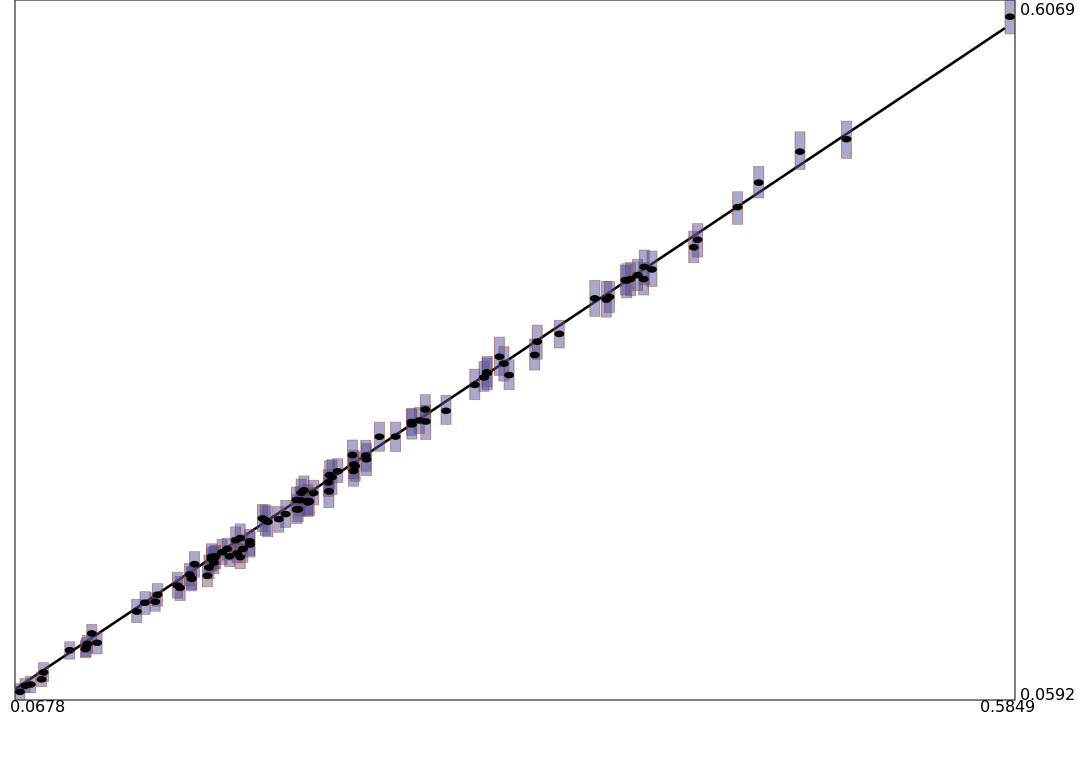
\includegraphics[width=0.19\textwidth]{../figures/bargraph-ok-strong}
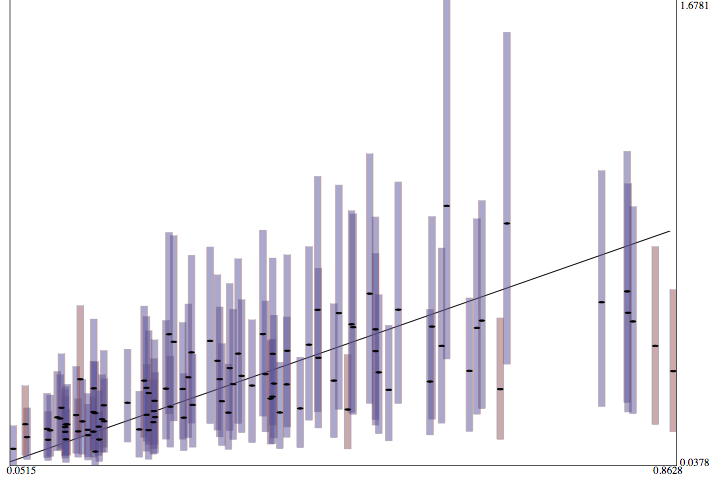
\includegraphics[width=0.19\textwidth]{../figures/bargraph-ok-medium}
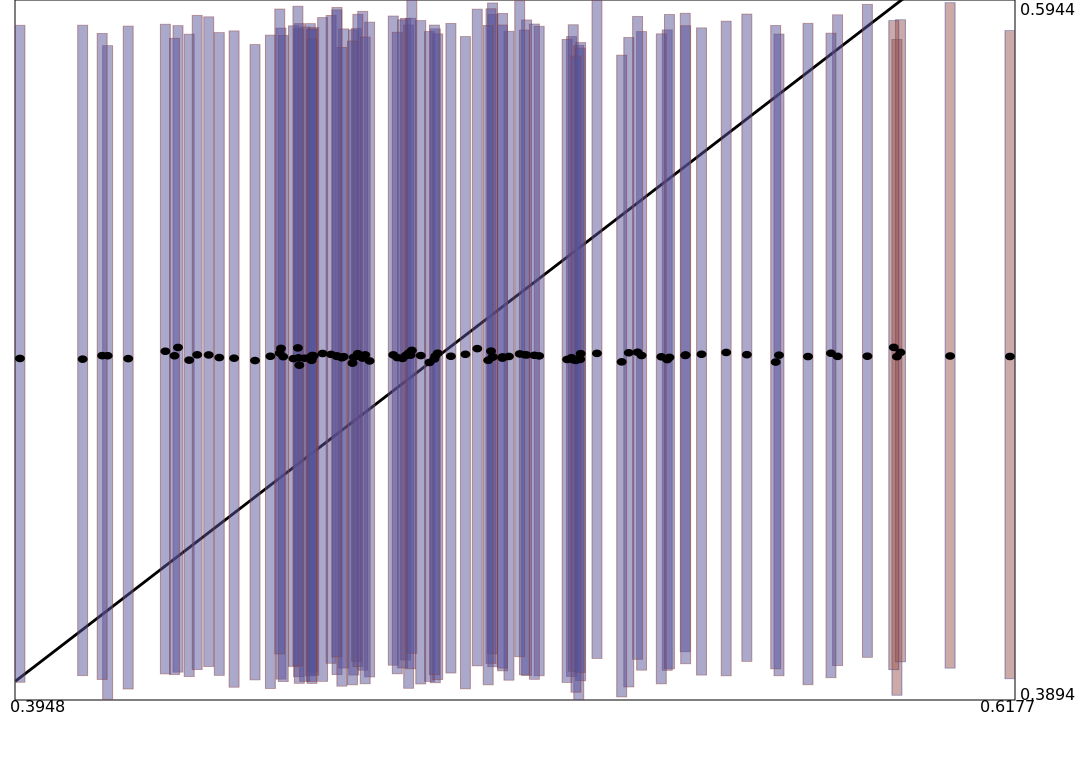
\includegraphics[width=0.19\textwidth]{../figures/bargraph-ok-weak}
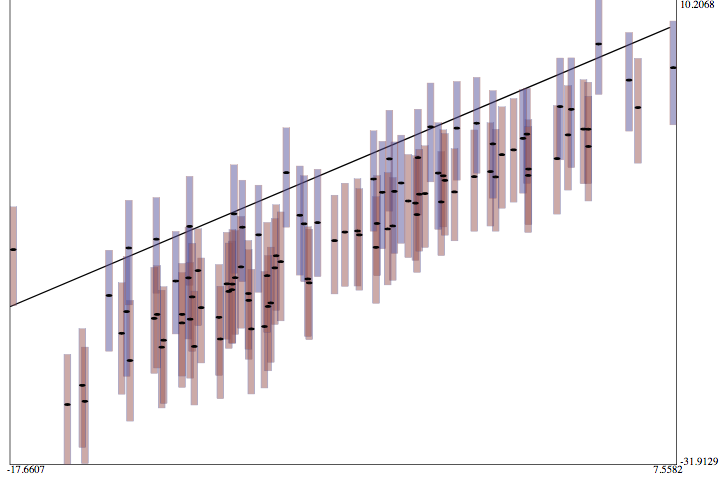
\includegraphics[width=0.19\textwidth]{../figures/bargraph-under}
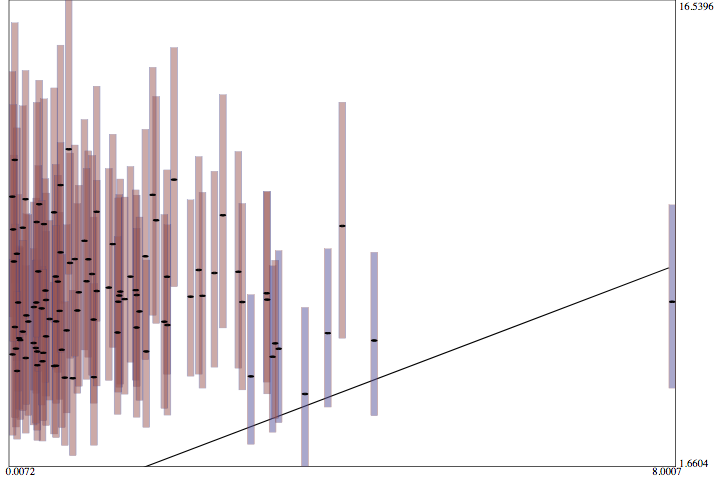
\includegraphics[width=0.19\textwidth]{../figures/bargraph-over}
\caption{\label{fig:coverage}
Graphs show true value on x-axis and estimates on y-axis. Black line shows where x equals y axis, and where ideally most of the probability mass is concentrated. Black dots are means of estimates. Bars indicate 95\% HPDs where blue bars cover the true value and red ones do not. Ideally 95 out of 100 bars should be blue.
a) Strong coverage: true parameter can be inferred accurately.
b) Medium coverage: true parameter can be inferred, but with high uncertainty.
c) Weak coverage: true parameter cannot be inferred, even though 95\% HPD covers the true value sufficiently often.
d) True parameter is over estimated.
e) True parameter is under estimated.
}
\end{figure}


\section{Setting priors}\label{setting-priors}

For a well calibrated test, priors need to be selected. Ideally, these priors should 
cover the widest range of possible applications. However, in many software implementations,
the priors are set so wide that when used in a well calibrated test, many parameters cannot
be recovered. Here, we provide some guidelines on how to set priors for some parameters
that are frequently occurring in phylogenetic models.

\subsection{Trees \& clock model
parameters}\label{trees-clock-model-parameters}

The mutation rate \(\mu\) must have been such that the tree height
\(h_T\) cannot exceed \(1/\mu\) (in other words, \(\mu h_T\le 1\)),
otherwise there would be saturation, and sequences could not possibly
have sufficient information to align. At the other end of the spectrum,
where \(\mu h_T\) close to zero, very long sequences are required to
ensure there are enough mutations in order to be able to reconstruct the
tree distribution.

% TODO: formulate in terms of \(N_e\) instead of \(h_T\)?

For reasonable computation times, trees should never be over 1 substitutions high
to prevent unreliable reconstruction of the phylogeny. Ideally, they should
be about 0.5 substitutions high and sequences of about 1000 base pairs long will be
sufficient. If a wider range is chose,  sequences may need to be much longer to reliably 
reconstruct smaller trees. Adding gamma rate heterogeneity to the model can alleviate 
the requirement for longer sequences somewhat, but having trees fairly close 

One way to enforce a range on the tree height is to have
 a narrow prior on birth rates (for birth/death type tree priors), or enforcing 
 it directly by  putting an MRCA prior on the height of the tree, for coalescent
 models. Note that the latter hampers direct simulator implementations.

For clock models with mean clock rate not equal to 1, simulate trees with clock
rates times tree height approximately 0.5.

Published mutation rates can range from \(O(1e-2)\) substitutions per
site per year for viruses such as HIV (\cite{cuevas2015extremely}), to
\(O(1e-11)\) for conserved regions of nuclear DNA (e.g PyrE2 locus in
Haloferax volcanii (\cite{lynch2010evolution})). So, for releases, tree priors for clock
and trees should be made less informative in order to cater for a wider 
range of tree heights and clock rates.

{\bf Gamma rate heterogeneity}\label{gamma-rate-heterogeneity}:
To prevent saturation, adding categories with slow rates will go some
way to allow covering a larger range of clock rates. Using gamma rate
heterogeneity with shape values in the range 0.1 to 1 allows this, so
adopt a gamma shape prior accordingly.

{\bf Proportion invariable sites}\label{proportion-invariable-sites}:
Since each site evolves with non-zero rate, use of proportion invariable
sites is modelling the process badly, and therefore not recommended.

{\bf Frequencies}\label{frequencies}:
Priors ideally should be set in realistic ranges, e.g.~frequency priors
not uniform(0,1) but Dirichlet(4,4,4,4) is better.

{\bf Substitution model parameters}\label{substitution-model-parameters}:
Default priors seem OK for most substitution models.



\section{Coverage trouble shooting}\label{trouble-shooting}

With 100 trials, the occasional 91 is acceptable (the 95\% HPD = 90 to 98 probability the
implementation is correct -- see Table \ref{tab:coverage}) but coverage below 90 almost surely indicate
an issue with the model or operator implementation. Also, coverage of 99
or 100 should be looked at with suspicion -- it may indicate overly wide
uncertainty intervals.


\begin{table}
\begin{center}
\begin{tabular}{rlll}
\hline
k & $p(x=k)$ & $p(x\le k)$ & $p(x\ge k)$\\
\hline
90 & 0.0167 & 0.0282 & 0.9718\\
91 & 0.0349 & 0.0631 & 0.9369\\
92 & 0.0649 & 0.1280 & 0.8720\\
93 & 0.1060 & 0.2340 & 0.7660\\
94 & 0.1500 & 0.3840 & 0.6160\\
95 & 0.1800 & 0.5640 & 0.4360\\
96 & 0.1781 & 0.7422 & 0.2578\\
97 & 0.1396 & 0.8817 & 0.1183\\
98 & 0.0812 & 0.9629 & 0.0371\\
99 & 0.0312 & 0.9941 & 0.0059\\
100 & 0.0059 & 1.0000 & 0.0000\\
\hline
\end{tabular}
\end{center}
\caption{If correctly implemented, the number of items covered is distributed binomial with p=0.95, N=100.
Source \url{https://www.di-mgt.com.au/binomial-calculator.html}.
\label{tab:coverage}}
\end{table}



Common causes of low coverage are ESS too low,
trees cannot be reconstructed reliably (height should not be too small or large),
Hastings ratio in operators incorrectly implemented, and
bugs in model likelihood implementation.
So, the first thing to check when coverage is too low, is the ESS used for
estimates.
One reason coverage can be lower is if the ESSs are too small, which can
be easily checked by looking at the minimum ESS for the log entry. If
these values are much below 200 the chain length should be increased to
be sure any low coverage is not due to insufficient convergence of the
MCMC chain.




\vspace{1cm}

\noindent [Well-calibrated validation: coverage, correlation between truth and
mean posteriors]

\vspace{1cm}

\noindent [Table: Bayesian packages that have (or not) done well-calibrated
validation studies]






% \section{Stats tricks for validating models}


% For a density $p$ on data $x$ (this could be a scalar, vector, or a tree) parameterised by the vector $\theta$, the expected value of the score function $U(\theta,x)=\frac{\partial}{\partial\theta}\log p(x;\theta)$ is 0:

% \begin{equation}\label{eq:scorefunction}
% E(U(\theta,x)) = \int U(\theta,x)p(x;\theta)dx = 0
% \end{equation}

% (this is the expected value over the data $x$ at the true parameters $\theta$). Also, the covariance of the score function is equal to the negative Hessian of the log-likelihood:

% $$
% \textrm{Var}(U(\theta, x))=-E\left(\frac{\partial^2}{\partial\theta^2}\log p(x;\theta)\right)
% $$

% Or equivalently:

% \begin{equation}\label{eq:variancestatistic}
% E\left(U(\theta, x)U(\theta, x)^T + \frac{\partial^2}{\partial\theta^2}\log p(x;\theta)\right)=0 
% \end{equation}

% Proofs of these results are relatively straightforward\footnote{\url{https://en.wikipedia.org/wiki/Score_(statistics)}}. The proofs depend on some regularity conditions to interchange integration and differentiation\footnote{\url{https://en.wikipedia.org/wiki/Leibniz_integral_rule}}; roughly speaking, the parameters must not change the support of the data. This means they don't hold for some parameters of interest in phylogenetics e.g. the origin time in a birth-death tree prior.

% These properties can be used in conjunction with a direct simulator as a necessary but not sufficient check that the likelihood is implemented correctly. The score function (\ref{eq:scorefunction}) and Hessian (\ref{eq:variancestatistic}) statistics can be calculated on samples from the simulator and a hypothesis test used to check that their mean is 0. In the multivariate case a potentially useful test is the likelihood ratio test for a multivariate normal with zero mean. If there are non-identifiable parameters there may be issues with performing this test as colinearity will lead to a singular sample covariance matrix.

% In practice it is appropriate to compute the score function by calculating derivatives using finite differences\footnote{Implemented here: \url{https://github.com/christiaanjs/beast-validation/blob/master/src/beast/validation/statistics/NumericalScoreFunctionStatistics.java}}.

% \subsection{Comparing multivariate distributions}

% Often we want to evaluate whether two multivariate samples are drawn from the same distribution. For example, when testing that an MCMC sampler produces the same distribution as direct simulation. There is no obvious choice of statistical machinery for performing this test. A popular univariate test for whether two samples are drawn from the same distributions is the Kolmogorov-Smirnov (KS) test\footnote{\url{https://en.wikipedia.org/wiki/Kolmogorov\%E2\%80\%93Smirnov_test\#Two-sample_Kolmogorov\%E2\%80\%93Smirnov_test}}, which uses a statistic based on the maximum difference between empirical cumulative distribution functions (ECDFs). The asymptotic distribution of this statistic has been derived. One way to adapt this to multivariate samples would be to test the marginals, but this would miss differences in correlations between variables.

% We can extend this test to multivariate distributions using multivariate ECDFs\footnote{\url{https://en.wikipedia.org/wiki/Cumulative_distribution_function\#Multivariate_case}}. However, the asymptotic distribution of this statistic is not known. One approach would be to generate a sampling distribution of the statistic under the null hypothesis (distributions being the same) with the non-parameteric bootstrap, pooling samples from both distributions. Calculating the ECDF for each bootstrap sample is expensive but can be made more efficient by pre-computing indicators of pairwise 'less than's between samples\footnote{Implemented here: \url{https://github.com/christiaanjs/beast-validation/blob/master/src/beast/validation/tests/BootstrapMultivariateDistributionTest.java}}.

\section*{Concluding remarks}

When publishing well calibrated studies, all XML files, log files and
scripts for manipulating them should be made available, so the study can
be replicated exactly as is. A practical way to do this is through a
\href{http://github.com}{github} repository.

Version numbers of BEAST and packages used should be noted.

For released software, default priors should be made as uninformative as 
possible and/or provide some guidance on how to set them -- users will use defaults.

\subsection*{Funding}
F.K.M. and A.J.D. were supported by Marsden grant 16-UOA-277. R.B. was
supported by Marsden grant .


%----------------------------------------------------------------------------------------
%	REFERENCE LIST
%----------------------------------------------------------------------------------------

% \section*{References}
% \clearpage

\bibliography{refs}

%----------------------------------------------------------------------------------------

\end{document}
